%\lstset{language=[Sharp]C}
\chapter{Allgemeines}
Shulker-Mobile ist eine Mobile-Applikation zur Steuerung des Türschlosses.
Shulker-Mobile wurde in \nameref{flutter} entwickelt.
Die Funktionalität von Shulker-Mobile beinhaltet das öffnen bzw. schließen des Türschlosses und das
erstellen neuer Pins, die am Touchscreen des Türschlosses verwendet werden können, um dieses zu öffnen.

\section{Verbinden des Türschlosses}
Beim ersten Start der Applikation muss sich diese die Verbindungsparameter für die Kommunikation mit dem Türschloss speichern.
Für diesen Vorgang bietet Shulker-Mobile 2 Möglichkeiten:
\begin{itemize}
    \item Türschloss manuell verbinden
    \item Türschloss mittels QR-Code verbinden
\end{itemize}
Nachdem der Nutzer das Türschloss erstmalig verbunden hat, werden die Verbindungsparameter über das 
\textit{shared\_preferences}-Paket lokal auf dem Smartphone gespeichert. 

\begin{figure}[H]
    \begin{center}
        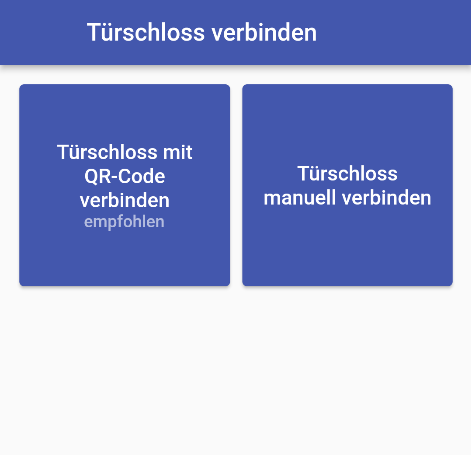
\includegraphics[width=.5\textwidth]{images/mobile/ConnectLockOptions.png}
        \caption{Optionen zum verbinden des Türschlosses}
    \end{center}
\end{figure}

\subsection{Türschloss manuell verbinden}
Um die Applikation manuell mit dem Türschloss zu verbinden, muss sowohl die lokale IP-Adresse des Raspberry PI's, als
auch der Port des vom Shulker-Connect laufenden Web-Servers angegeben werden.

\begin{figure}[H]
    \begin{center}
        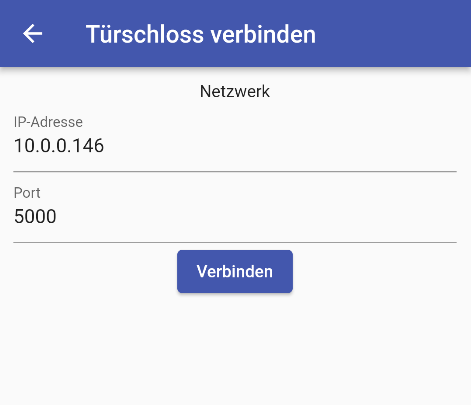
\includegraphics[width=.5\textwidth]{images/mobile/ManualConnect.png}
        \caption{Eingabefelder um das Türschloss manuell zu verbinden}
    \end{center}
\end{figure}

\subsection{Türschloss mittels QR-Code verbinden}
Alternativ stellt das Shulker-Türschloss-System auch eine leichtere, empfohlene Option, bereit, um die App mit dem Türschloss
zu verbinden.

toDo: Bild einfügen

Hierzu kann der Nutzer auf dem Touchscreen des Türschlosses einen QR-Code anzeigen lassen, welche die Verbindungsparameter
beinhaltet und in der App gescannt werden kann. Die ausgelesenen Daten werden dann automatisch in das gleiche Formular,
das auch bei der manuellen Verbindung verwendet wird, eingefügt. So muss der Nutzer keine Verbindungsparameter manuell
in die App eintragen.

\subsection{Verbindung außerhalb des Lokalen Netzwerkes}
Natürlich soll das Türschloss nicht nur vom Lokalen Netzwerk des Raspberry PI's, sondern auch vom Internet aus 
gesteuert werden können.
Um dies zu ermöglichen, muss auf dem Router des Heimnetzes ein VPN-Server eingerichtet werden.
Da die Konfiguration eines VPN-Servers von Router zu Router unterschiedlich ist, gehen wir auf dies nicht genauer ein.
Im Internet finden sich viele Anleitungen, die dies für diverse Router erklären.
\pagebreak
\subsubsection{Überprüfung der Verbindung in der Applikation}
Beim Start der Applikation müssen einige Dinge überprüft werden, um sicherzustellen, dass die Kommunikation mit 
dem Türschloss reibungslos funktioniert. Dies ist in folgendem Ablaufdiagramm ersichtlich:
\begin{figure}[H]
    \begin{center}
        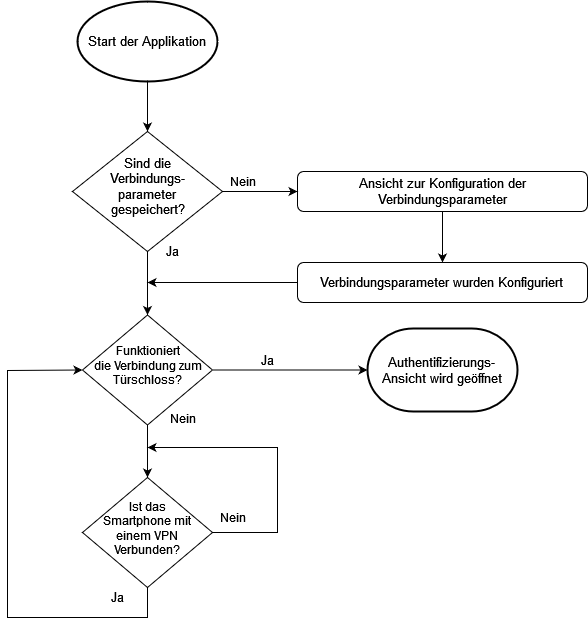
\includegraphics[width=0.8\textwidth]{images/mobile/Startup.png}
        \caption{Workflow um eine Verbindung zum Türschloss herzustellen}
    \end{center}
\end{figure}
Als erstes überprüft die Applikation nach ihrem Start, ob die Verbindungsparameter bereits lokal gespeichert sind.
Ist das nicht der Fall, öffnet sich die Ansicht, um die Verbindungsparameter zu konfigurieren.

Im zweiten Schritt sendet die Applikation eine Testanfrage an die \textit{/api/Status} Route, um die Verbindung 
zum Türschloss zu überprüfen.
Befindet sich das Smartphone aktuell im selben Netzwerk wie der Raspberry PI, wird diese Testanfrage erfolgreich sein, 
und somit kann nun der Authentifizierungs-Bildschirm geöffnet werden.
\pagebreak
Falls diese Anfrage scheitert, und sich das Smartphone somit nicht im Heimnetzwerk befindet, 
wird nun eine Ansicht geöffnet, in der der Nutzer mittels eines Buttons
die Smartphone-Einstellungsseite öffnen kann, in der die aktive VPN-Verbindung verwaltet werden kann.
Die App überprüft währenddessen laufend, ob sich der Nutzer mit einem VPN Verbunden hat.
In diesem Fall überprüft die Applikation anschließend wieder die Verbindung mittels einer Testanfrage. 

\subsection{Authentifizierung bei Start der App}
Nachdem die App eine Verbindung zum Türschloss sichergestellt hat, öffnet sich die Authentifizierungs-Ansicht.
Dort wird der User aufgefordert, das Master-Passwort des Türschlosses einzugeben.

\begin{figure}[H]
    \begin{center}
        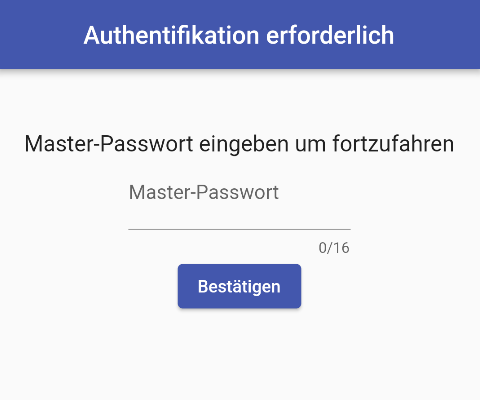
\includegraphics[width=.5\textwidth]{images/mobile/AuthScreen.png}
        \caption{Ansicht zur Authentifikation.}
    \end{center}
\end{figure}

Das eingegebene Master-Passwort wird dazu verwendet, um auf der \textit{/api/Session/getToken/\{secret\}}-Route
eine neue Session anzufragen. Zusätzlich dient diese Eingabe auch als Schutz der App vor unbefugtem Zugriff.
Die App ist somit kein Angriffsvektor, da ohne eine aktive Session keine Befehle an das Türschloss gesendet werden können.
\pagebreak
\subsection{Startbildschirm}
Der Startbildschirm der Applikation wird nach erfolgreichem anfragen der Session aufgerufen.
Dort lässt sich das Türschloss jederzeit öffnen bzw. schließen.
Nachdem das Türschloss geöffnet wurde, bleibt es 24 Sekunden geöffnet, bevor es sich wieder automatisch schließt.
Links befindet sich ein kleiner Knopf, mit dem eine Sidebar geöffnet werden kann, welche weitere Ansichten öffnen kann.

\begin{figure}[H]
    \begin{center}
        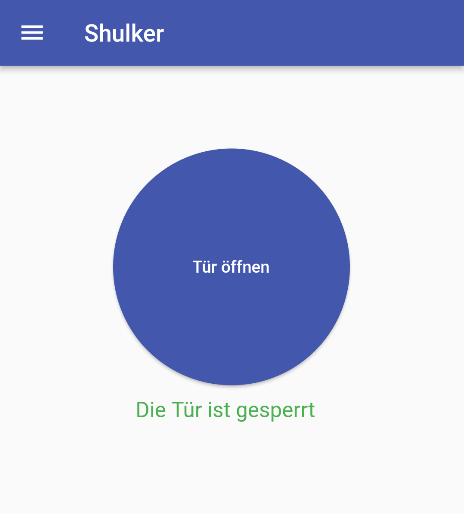
\includegraphics[width=.5\textwidth]{images/mobile/Homescreen.png}
        \caption{Der Startbildschirm von Shulker-Mobile.}
    \end{center}
\end{figure}
\pagebreak
\subsection{Sidebar}
Die Sidebar öffnet sich links am Bildschirm und gibt eine Übersicht der verschiedenen Ansichten,
die geöffnet werden können.

\begin{figure}[H]
    \begin{center}
        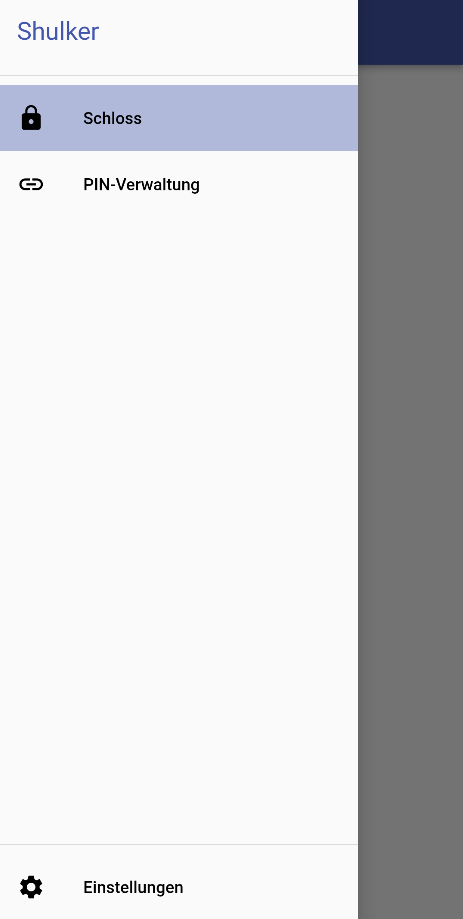
\includegraphics[width=.5\textwidth]{images/mobile/Sidenav.png}
        \caption{Die Sidebar listet verschiedene Ansichten von Shulker-Mobile an.}
    \end{center}
\end{figure}
\pagebreak
\subsection{PIN-Verwaltung}
Die PIN-Verwaltungs-Ansicht bietet einen Überblick aller erstellten Pins.

\begin{figure}[H]
    \begin{center}
        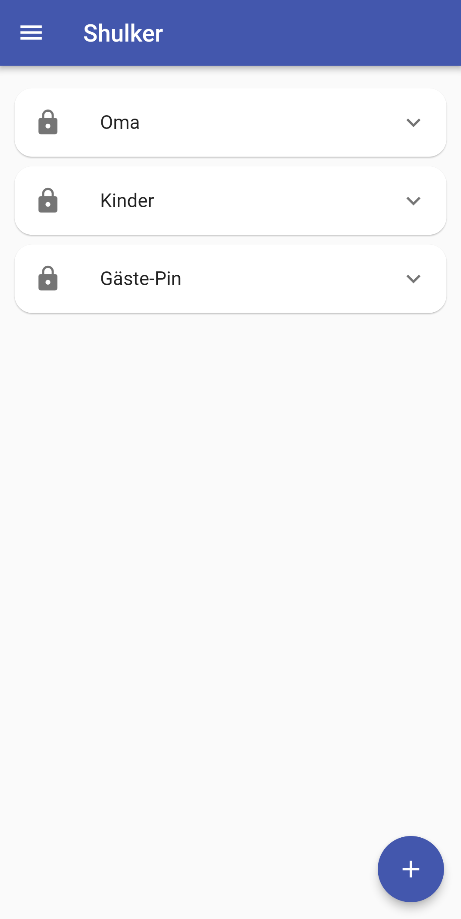
\includegraphics[width=.5\textwidth]{images/mobile/PinManager.png}
        \caption{Die PIN-Verwaltungs-Ansicht von Shulker-Mobile}
    \end{center}
\end{figure}

Einzelne Pins können angeklickt werden, um weitere Informationen über diese anzuzeigen.
Nachdem ein Pin angeklickt wurde, öffnet sich dieser.
Nun lässt sich auslesen, wie oft dieser Pin noch verwendet werden kann, und in welchem 
Zeitraum dieser gültig ist.
Außerdem lassen sich Pins von diesem Menü aus löschen.

\begin{figure}[H]
    \begin{center}
        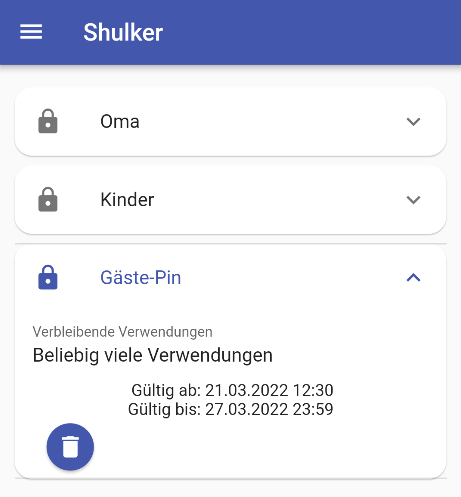
\includegraphics[width=.5\textwidth]{images/mobile/ClickedPin.png}
        \caption{Geöffnetes Menü, nachdem ein Pin angeklickt wurde.}
    \end{center}
\end{figure}

\subsection{Erstellen eines Pins}
In der rechten unteren Ecke der PIN-Verwaltungs-Ansicht befindet sich ein \textit{Floating Action Button},
der ein Fenster öffnet, um neue Pins zu erstellen.

\begin{figure}[H]
    \begin{center}
        
\includegraphics[width=.1\textwidth]{images/mobile/CreatePinButton.png}
        \caption{Knopf zum erstellen eines Pins}
    \end{center}
\end{figure}

Nachdem dieser gedrückt wurde, öffnet sich ein Fenster, das einem Formular beinhaltet, um neue Pins zu erstellen.

\begin{figure}[H]
    \begin{center}
        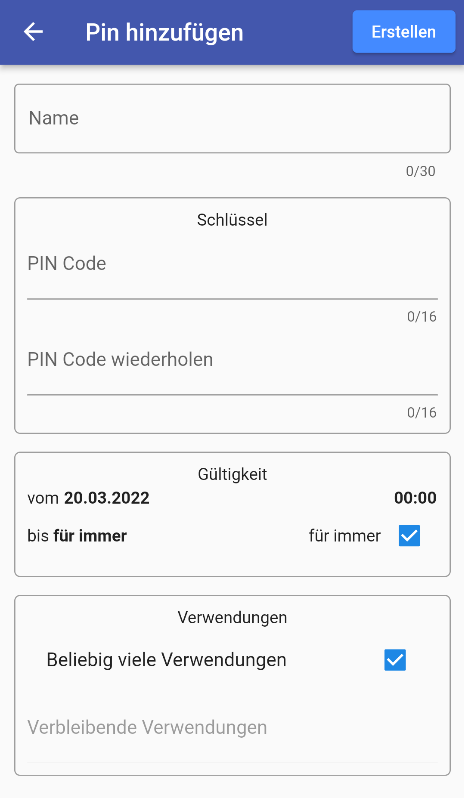
\includegraphics[width=.5\textwidth]{images/mobile/CreatePin.png}
        \caption{Fenster zum erstellen eines Pins}
    \end{center}
\end{figure}

Dort muss dem Pin einen Namen gegeben werden.
Dann kann der Schlüssel des Pins eingetragen werden, dieser muss zwei mal eingegeben werden, um sicherzustellen,
dass sich der Nutzer bei der Eingabe nicht verschrieben hat.
Alle Felder dieses Formulars beinhalten eine Validierung der Eingabe.

Zusätzlich kann dort noch die Gültigkeit und die Anzahl der Verwendungen angegeben werden.
Um einen Zeitpunkt für die Gültigkeit zu definieren, muss dieser einfach angeklickt werden.
Anschließend öffnet sich ein Fenster, in dem Datum bzw. Uhrzeit ausgewählt werden kann.
Nachdem ein Pin hinzugefügt wurde, erscheint dieser in der Pin-Verwaltungs-Ansicht.

\begin{figure}[H]
    \begin{center}
        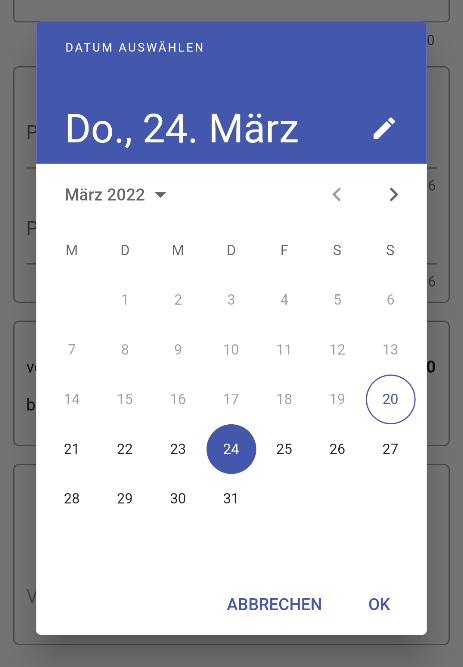
\includegraphics[width=.4\textwidth]{images/mobile/DatePicker.png}
        \caption{Fenster zur Auswahl eines Datums. }
    \end{center}
\end{figure}

\begin{figure}[H]
    \begin{center}
        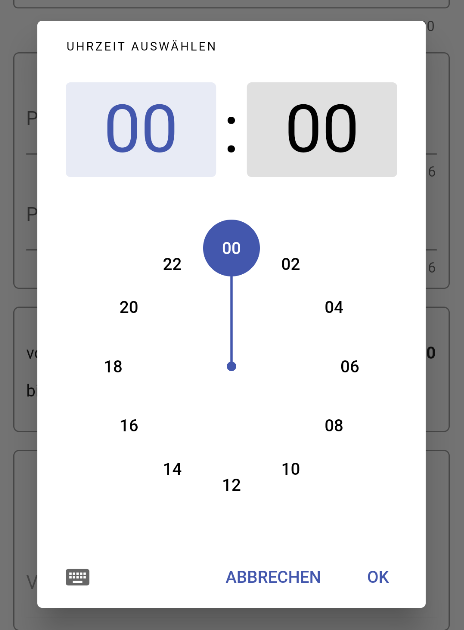
\includegraphics[width=.4\textwidth]{images/mobile/TimePicker.png}
        \caption{Fenster zur Auswahl einer Uhrzeit.}
    \end{center}
\end{figure}

\subsection{Einstellungen}
\begin{figure}[H]
    \begin{center}
        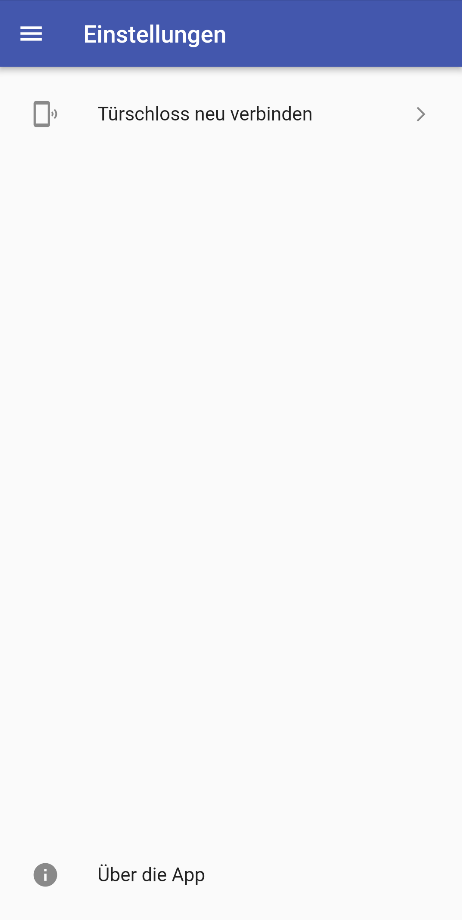
\includegraphics[width=.4\textwidth]{images/mobile/Settings.png}
        \caption{Einstellungs-Ansicht}
    \end{center}
\end{figure}

Die Einstellungs-Ansicht ist von der Sidebar aus aufrufbar. Dort befindet sich ein Knopf, um das Türschloss neu
zu Verbinden, und ein weiterer, um Informationen über die App, wie Versionsnummer und Lizenzen der verwendeten
Software, anzuzeigen.

\begin{figure}[H]
    \begin{center}
        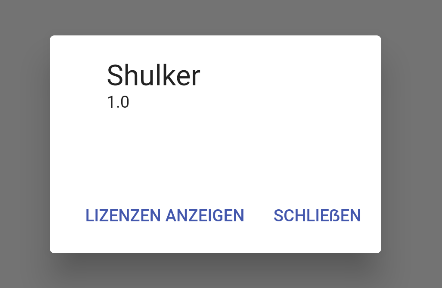
\includegraphics[width=.4\textwidth]{images/mobile/AboutTheApp.png}
        \caption{Fenster, dass Informationen über die App anzeigt. Wird von Flutter bereitgestellt. }
    \end{center}
\end{figure}

Das Menü, dass nach einem Klick auf den „Über die App“-Knopf aufgerufen wird, wird von Flutter bereitgestellt.
Der Knopf „Lizenzen Anzeigen“ listet die Lizenzen der im Projekt verwendeten Software. 

\begin{figure}[H]
    \begin{center}
        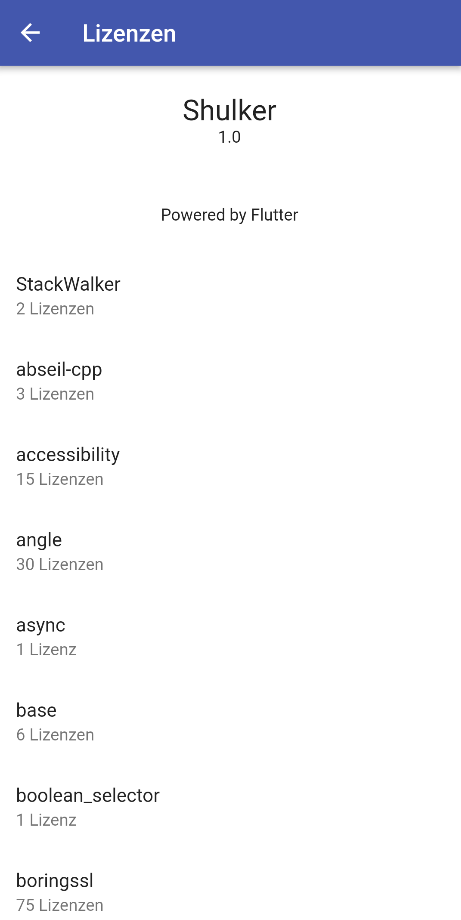
\includegraphics[width=.4\textwidth]{images/mobile/Licences.png}
        \caption{Fenster, dass alle verwendeten Software-Komponenten und dessen Lizenzen anzeigt. 
        Wird von Flutter bereitgestellt. }
    \end{center}
\end{figure}